
\documentclass[10pt]{article}
% \usepackage[letterpaper,text={6.5in,8.7in},centering]{geometry}
\usepackage{amssymb,amsmath,times,url,graphicx,amsthm,alltt}
%\usepackage[pdftex,urlcolor=blue,pdfpagemode=none,pdfstartview=FitH]{hyperref}
\usepackage{my_packages}
\usepackage{tikz_packages}
%% url smaller font.
\makeatletter
\def\url@leostyle{%
\@ifundefined{selectfont}{\def\UrlFont{\sf}}{\def\UrlFont{\small\ttfamily}}}
\makeatother
\urlstyle{leo}

%\usepackage[all,import]{xy}

\renewcommand{\baselinestretch}{1.2}
\date{}

\renewcommand{\thesubsection}{\arabic{subsection}. }
\renewcommand{\thesubsubsection}{\arabic{subsection}.\arabic{subsubsection} }

\theoremstyle{definition}
\newtheorem{prob}{Problem}[section]
%\renewcommand{\theprob}{\arabic{section}.\arabic{prob}}
\renewcommand{\theprob}{\arabic{prob}}

\newenvironment{subprob}%
{\renewcommand{\theenumi}{\alph{enumi}}\renewcommand{\labelenumi}{(\theenumi)}\begin{enumerate}}%
{\end{enumerate}}%


\begin{document}

\pagestyle{empty}
\section*{MAE3134: Homework 5}
\vspace*{-0.4cm}
\noindent{Due date: }%\\%\vspace*{0.5cm}

\begin{prob}
    For each of the electrical systems below, find the state space representation.
    \begin{subprob}
    \item There is a single voltage source and the output is the voltage difference across the capacitor \( C_1 \).
        \begin{figure}[h]
            \centering
            \begin{scaletikzpicturetowidth}{0.8\textwidth}
                \begin{tikzpicture}[scale=\tikzscale]
                    \draw (0,0) to[american voltage source,v<=\( u(t)\)] (0,2) 
                        to[resistor, l^=$R_1$] (2,2) to[inductor, l=$H_1$] (2,0) 
                        to[short] (0,0); 
                    \draw (2, 2) to[resistor, l^=$R_2$] (4, 2) to[inductor, l=$H_2$] (4, 0) to[short] (2, 0);
                    \draw (4, 2) to[resistor, l=$R_3$] (6, 2) to[capacitor, l=$C_1$] (6, 0) to[short] (4, 0);
                \end{tikzpicture}
            \end{scaletikzpicturetowidth}

            \caption{Electrical System}
        \end{figure}

    \item The output is \( i(t) \), which defines the current across the resistor \( R_2\). 
        \begin{figure}[h]
            \centering
            \begin{scaletikzpicturetowidth}{0.8\textwidth}
                \begin{tikzpicture}[scale=\tikzscale]
                    \draw (0,0) to[american voltage source,v<=\( u_1(t)\)] (0,2) 
                        to[inductor, l^=$R_1$] (2,2) to[capacitor, l=$H_1$] (2,0) 
                        to[short] (0,0); 
                    \draw (2, 2) to[capacitor, l^=$H_1$] (4, 2) to[american voltage source, l=$u_2(t)$] (4, 0) to[short] (2, 0);
                    \draw (4, 2) to[short] (6, 2) to[resistor, l=$R_2$] (6, 0) to[short] (4, 0);
                \end{tikzpicture}
            \end{scaletikzpicturetowidth}
        \end{figure}
    \item The output is \( v_o(t) \) which defines the voltage across the resistor \( R_3\).
        \begin{figure}[h]
            \centering
            \begin{scaletikzpicturetowidth}{0.5\textwidth}
                \begin{tikzpicture}[scale=\tikzscale]
                    \draw (0,0) to[american voltage source,v<=\( u_1(t)\)] (0,2) 
                        to[resistor, l^=$R_1$] (2,2) to[capacitor, l=$H_1$] (2,0) 
                        to[short] (0,0); 
                    \draw (2, 2) to[capacitor, l^=$H_2$] (4, 2) to[resistor, l=$R_3$] (4, 0) to[short] (2, 0);
                    \draw (0, 2) to[short] (0, 4) to[resistor, l=$R_2$] (4, 4) to[short] (4, 2);
                \end{tikzpicture}
            \end{scaletikzpicturetowidth}
            \caption{Electrical System}
        \end{figure}
    \end{subprob}
\end{prob}

\begin{prob}
    \begin{figure}[h]
        \centering
        \begin{scaletikzpicturetowidth}{1\textwidth}
            \begin{tikzpicture}[scale=\tikzscale]
            \draw (0, 0) node[inner sep=0] {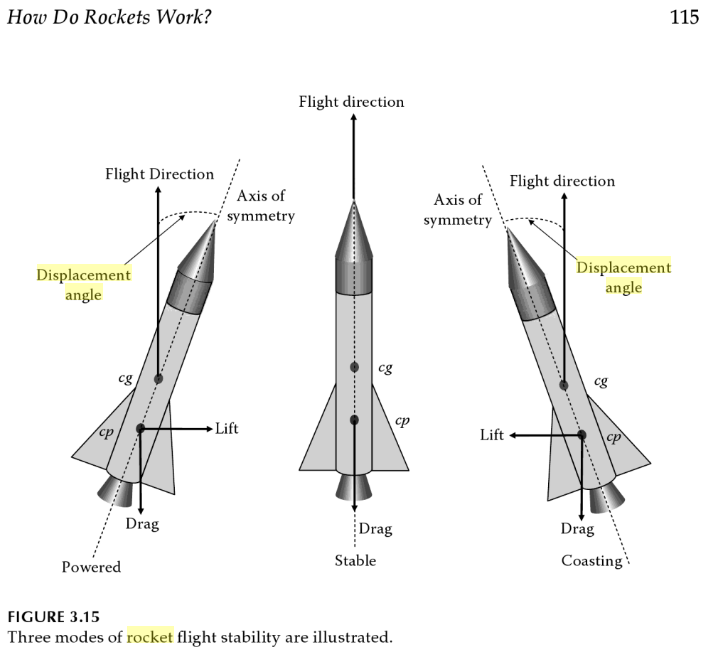
\includegraphics[width=0.7\textwidth]{figures/ArWeg.png}};
            \draw (-2, 1.4) node {\(\alpha\)};
        \end{tikzpicture}
    \end{scaletikzpicturetowidth}
    \caption{Missile in flight~\label{fig:missile}}
    \end{figure}
    A missile in flight, as shown in~\cref{fig:missile}, is subject to several forces: thrust, lift, draft, and gravity.
    The missile flies at an angle of attack \( \alpha \), from its longitutinaal axis, creating lift. 
    For steering, the body angle from vertical, \( \phi \), is controlled by rotating the engine at the tail. 
    The transfer function relating the body angle, \( \phi \), to the angular displacement \( \delta \) of the engine is of the form
    \begin{align*}
        \frac{\Phi(s)}{\delta(s)} = \frac{K_a s + K_b}{K_3 s^3 + K_2 s^2 + K_1 s + K_0}.  
    \end{align*}

    \noindent Find the representation of the missile steering control in state space.
\end{prob}

\clearpage\newpage
\begin{prob}
     \begin{figure}[h]
        \centering
        \subcaptionbox{F-4E with canards\label{fig:f4}}{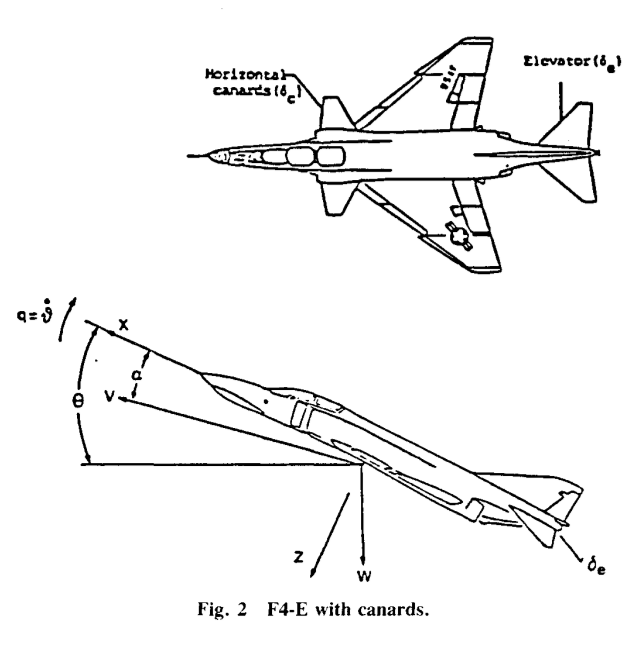
\includegraphics[width=0.5\textwidth]{figures/f4e.png}}~
        \subcaptionbox{F-4E in flight\label{fig:qf4e}}{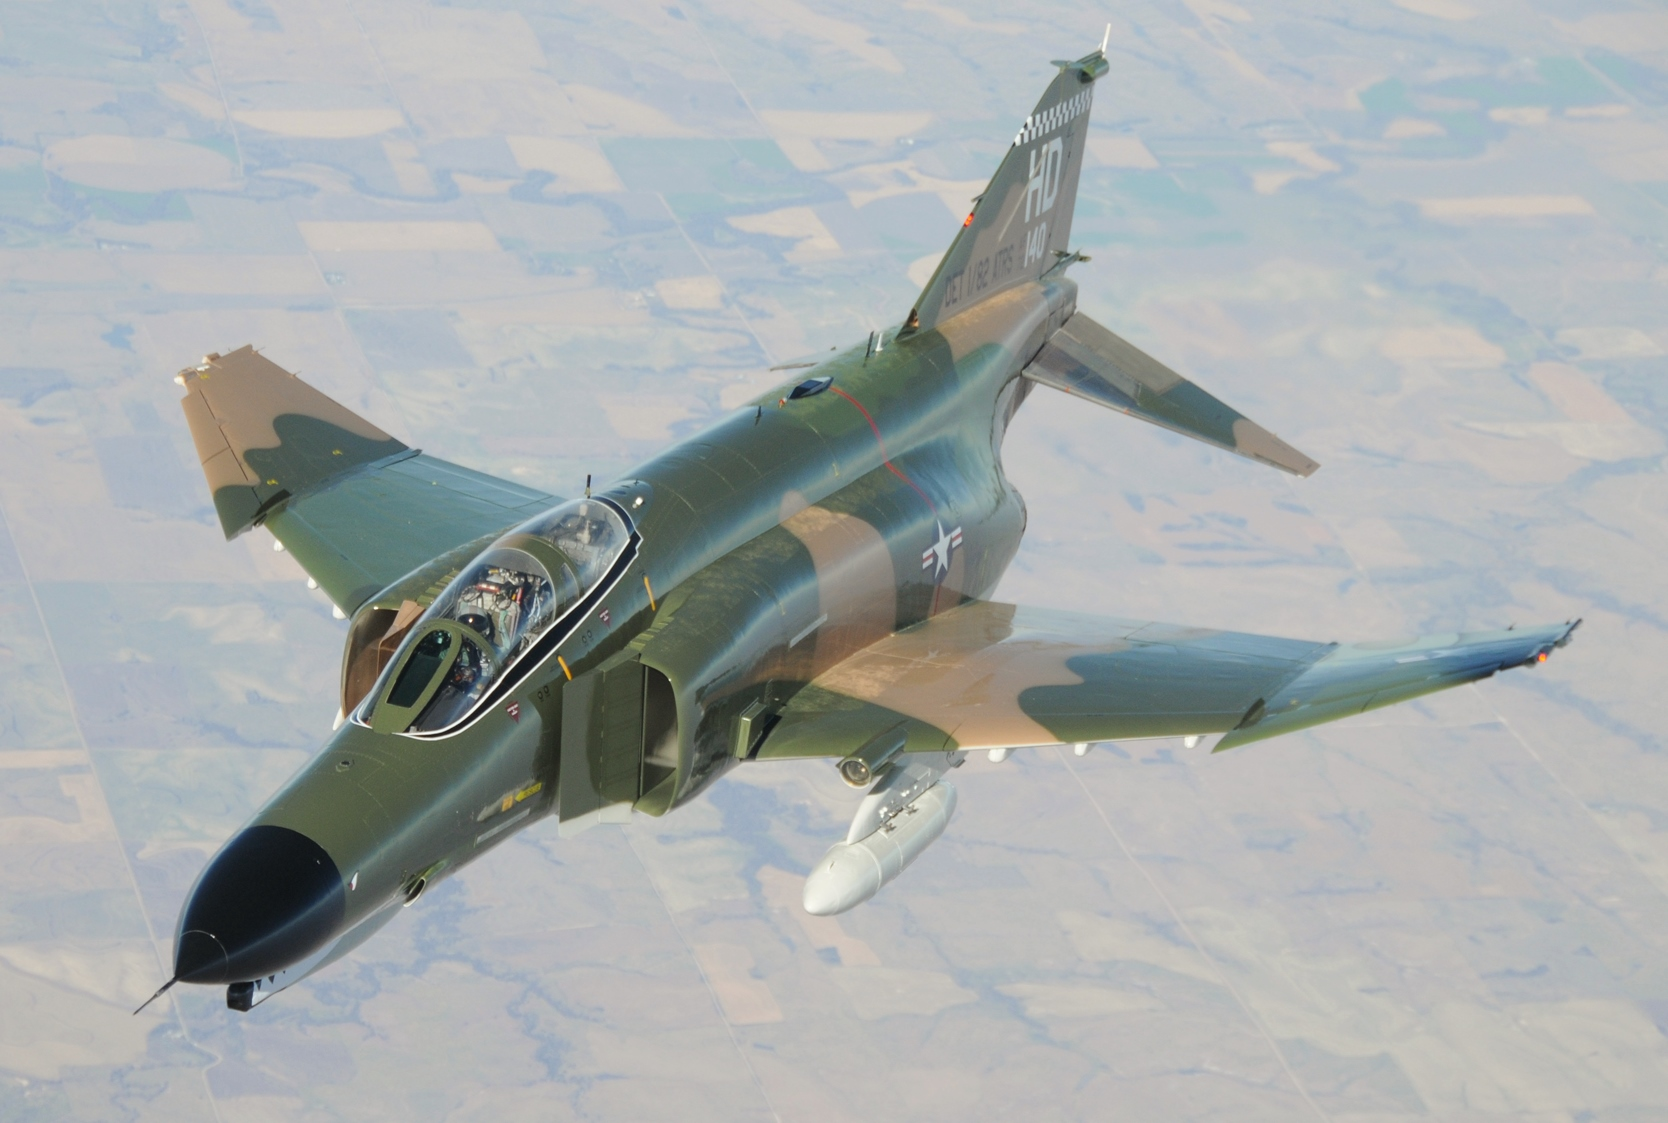
\includegraphics[width=0.5\textwidth]{figures/QF-4_Holloman_AFB.jpg}}
     \end{figure}
     The McDonnell Douglas F-4 Phantom II is a tandem two-seat, twin-engine, all-weather, long-range supersonic jet interceptor and fighter-bomber.
     First entering service in 1960, it proved highly adaptable and was a major part of the air wings of three service components, the US Navy, US Marine Corps and US Air Force.
     The F-4 was used extensively  during the Vietnam War and served as the principal air superiority fighter for both the Navy and Air Force.
     The F-4 remained in active use through the 1991 Gulf War serving in reconnaissance and Wild Weasel (Suppression of Enemy Air Defenses) roles.
    
     Normal accelerations, \( a_n \), and pitch rate, \( q \), are controlled by elevator deflection, \( \delta_e\), on the horizontal stabilizers and by canard deflection, \( \delta_c \).
    A commanded deflection , \( \delta_{com} \), is used to effect a change in both \( \delta_e \) and \( \delta_c\).
    The actuator deflections, combined with the aircraft longitudinal dynamics yield \( a_n \) and \( q\).
    The state equatinos describing the effect of \( \delta_{com} \) on \( a_n \) and \( q\) is given by
    \begin{align*}
        \begin{bmatrix} 
            \dot a_n \\ \dot q \\ \dot \delta_e 
        \end{bmatrix}
        = \begin{bmatrix}
            -1.702 & 50.72 & 263.38 \\
            0.22 & -1.418 & -31.99\\
            0 & 0 & -14
        \end{bmatrix}
        \begin{bmatrix}
            a_n \\ q \\ \delta_e
        \end{bmatrix}
        + 
        \begin{bmatrix}
            -272.06 \\ 0 \\14
        \end{bmatrix}
        \delta_{com} 
    \end{align*} .

    \noindent Find the following transfer functions:
    \begin{subprob}
        \item
            \[
                G_1(s) = \frac{A_n(s)}{\delta_{com}(s)}
            \]
        \item 
            \[
                G_2(s) = \frac{Q(s)}{\delta_{com}(s)}
            \]
    \end{subprob}
\end{prob}
\end{document}
